\subsection{Common Utilities}

This package contains the implementation of serializable classes which can be
exchanged among the client and the server in XML format. There are entities
classes that represents a simplification of the analysis classes.

Furthermore there are the \code{RequestMessage} and \code{ResponseMessage} which
are respectively representation of requests from the clients and responses from
the server.

These classes are composed by some fields which identifies the type of the
request and a set of \code{Entity} objects that are exchanged among the two
parties to fulfil the requests.

The diagram in Figure~\ref{fig:common} shows the implementation of these classes
and their interconnections.

\begin{landscape}
	\begin{figure}
		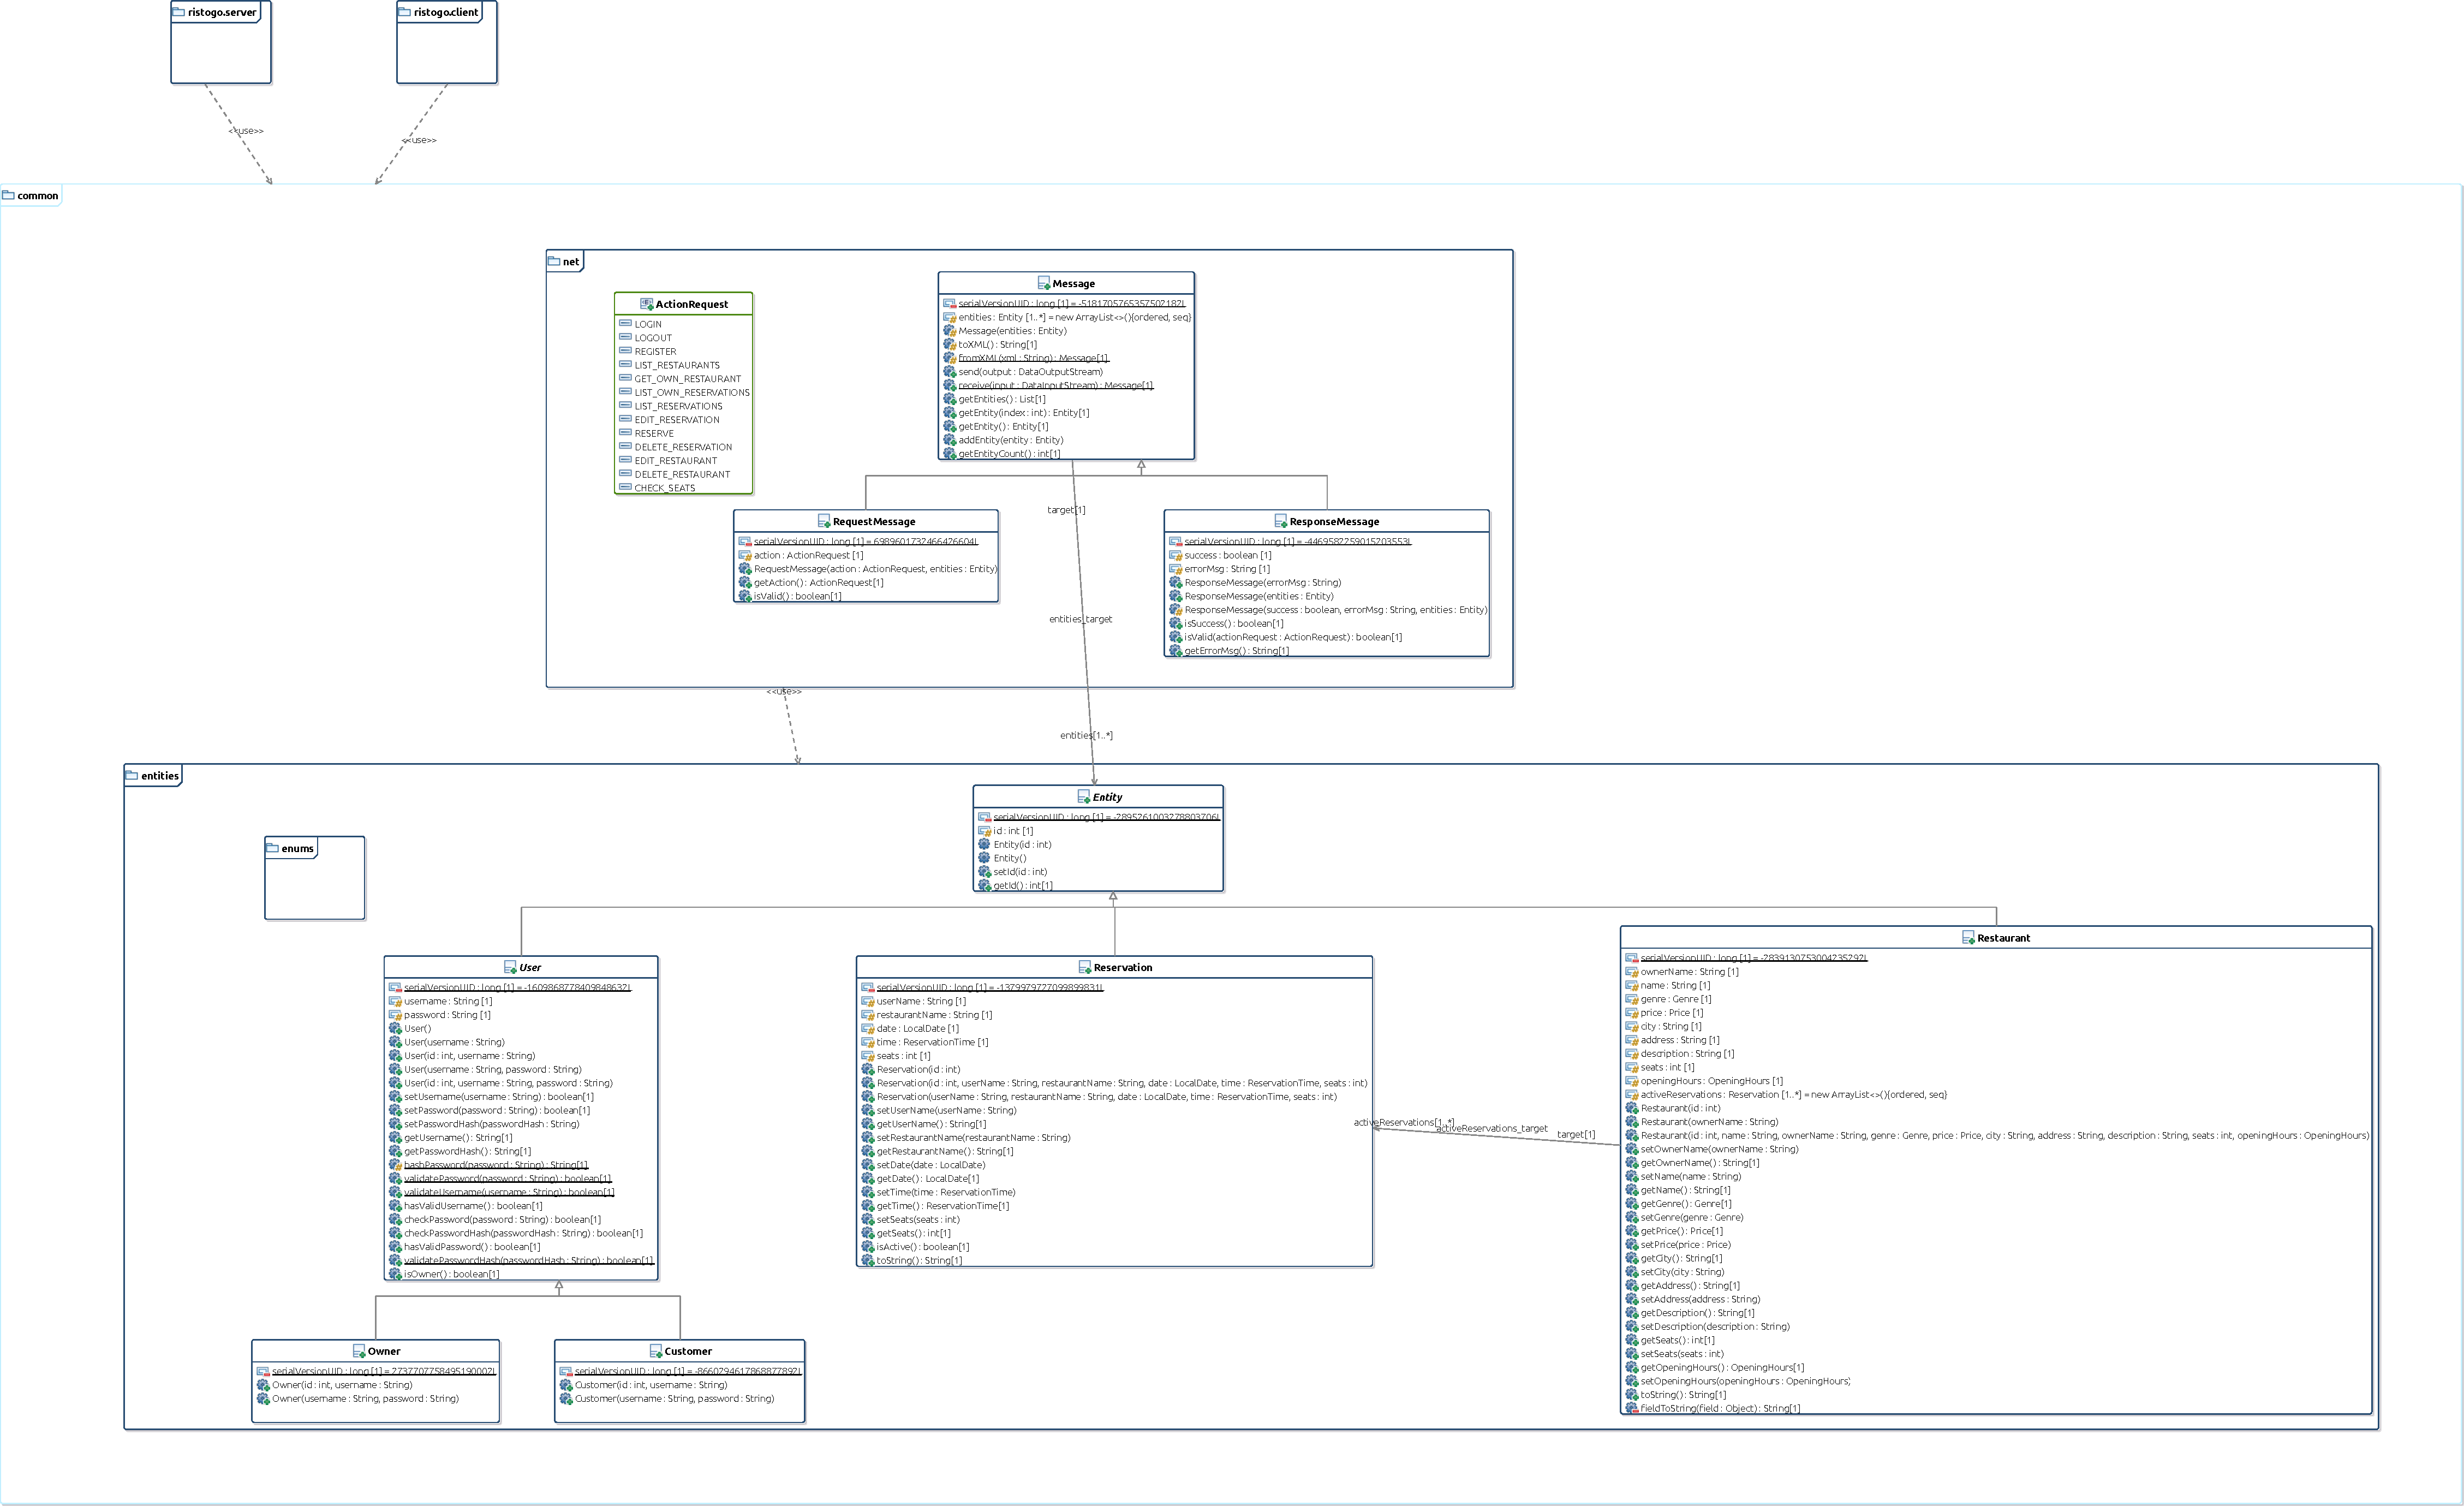
\includegraphics[width=0.8\paperheight]{common}
		\caption{\code{ristogo.common} UML Implementation Diagram.}
		\label{fig:common}
	\end{figure}
\end{landscape}
